\section{Computational Results}\label{sec:compResults}

In this section, we aim at studying mainly the recovery cost and the computing time of the CHARP for the overall thirty two data instances. Our experiments were conducted in an Intel Xeon Gold CPU @ 2.3GHz box which allowed to run simultaneously the overall data instances through the maximum delay time window in \ref{eq:timeWindow} :

\begin{equation}
	\begin{aligned}
		Time \: window = [720, 780, 840, 900, 960, 1020, 1080, 1140, 1200, 1260]
	\end{aligned}
	\label{eq:timeWindow}
\end{equation} 

Each of the values of \ref{eq:timeWindow} consist of the $maximumDelay$ parameter that is used in algorithm \ref{algo:flightDomains} to compute the flight domain.

The results for the aggregate cost are computed summing every data instance recovery cost and the computing time is measured when the last data instance finishes the recovery. We will also compute the total amount of delay, cancelled flights, new flights and, taxi flights necessary to recover the data instances.
 The remainder of this section consists of, Subsection \ref{sec:impact} where we will demonstrate the impact of adding new flights and taxi flights. Since the heuristic performs a pincer movement in Subsection \ref{sec:pincerSpeed} we will determine which is the best speed by changing the decremental and incremental steps. Finally in Subsection \ref{sec:stepSize} we will present the results for 20 and 35 minutes step size. \\
 
\subsection{Impact of New Flights and Taxi Flights}\label{sec:impact}
To study the impact of new flights we define the base scenario in table \ref{tbl:baseScenario}: 

	\begin{table}[h!]
		\centering
		\caption{Base Scenario}
		\label{tbl:baseScenario}
		\begin{tabular}{ll}
			\hline
			Domain step {[}min{]} & 60                           \\
			Upper bound           & $3.0 \times 10^{12}$ \\
			Upper bound step      & $1.0 \times 10^{11}$ \\
			Lower bound           & $4.0 \times 10^4$ \\
			Lower bound step      & $1.0 \times 10^4$ \\
			\hline
		\end{tabular}
	\end{table}

In  figure \ref{fig:flightNoFlight}, we represent the results for "Flights added" where we have both new flights and taxi flights to the CHARP, "No flights added" where the CHARP has no new or taxi flights added. "Only new flights added" and "Only taxi flight added", are self explanatory. We can observe that the aggregate cost is lower for the heuristic that has new flights and taxi flights added, than for the one with none of them added. This result was expected since adding new flights or taxi flights consists of adding new arcs which in turn can increase the flow of the flight network.\\
 We also observe in terms of aggregate cost that new fights have greater impact than new flights. It is possible to observe a similar results for the maximum time to obtain a solution. The latter can be explained on a series of cascading effects: adding new flights will decrease the available airport capacity, which in turn will decrease the size of the domains hence resulting in a smaller size search space which needs less time to be traversed.\\

 We  observe that extending the time window increases the total amount of delay returned by the CHARP. This results from that fact there are more time slots available to move the flight.\\
 
  As for the total number of cancellations we verify that it is lower for the heuristic that has new flights and taxi flights added, than for the one with none of them added. The tendency of this results is consistent with the aggregate cost. \\
  
   Finally we point out that the total number of new flights is in the order of magnitude of 125 and the total number of taxi flights is in the order of magnitude of 200. Both values do not change substantially with the size of the time window.

	\begin{figure}[h!]
		\centering
		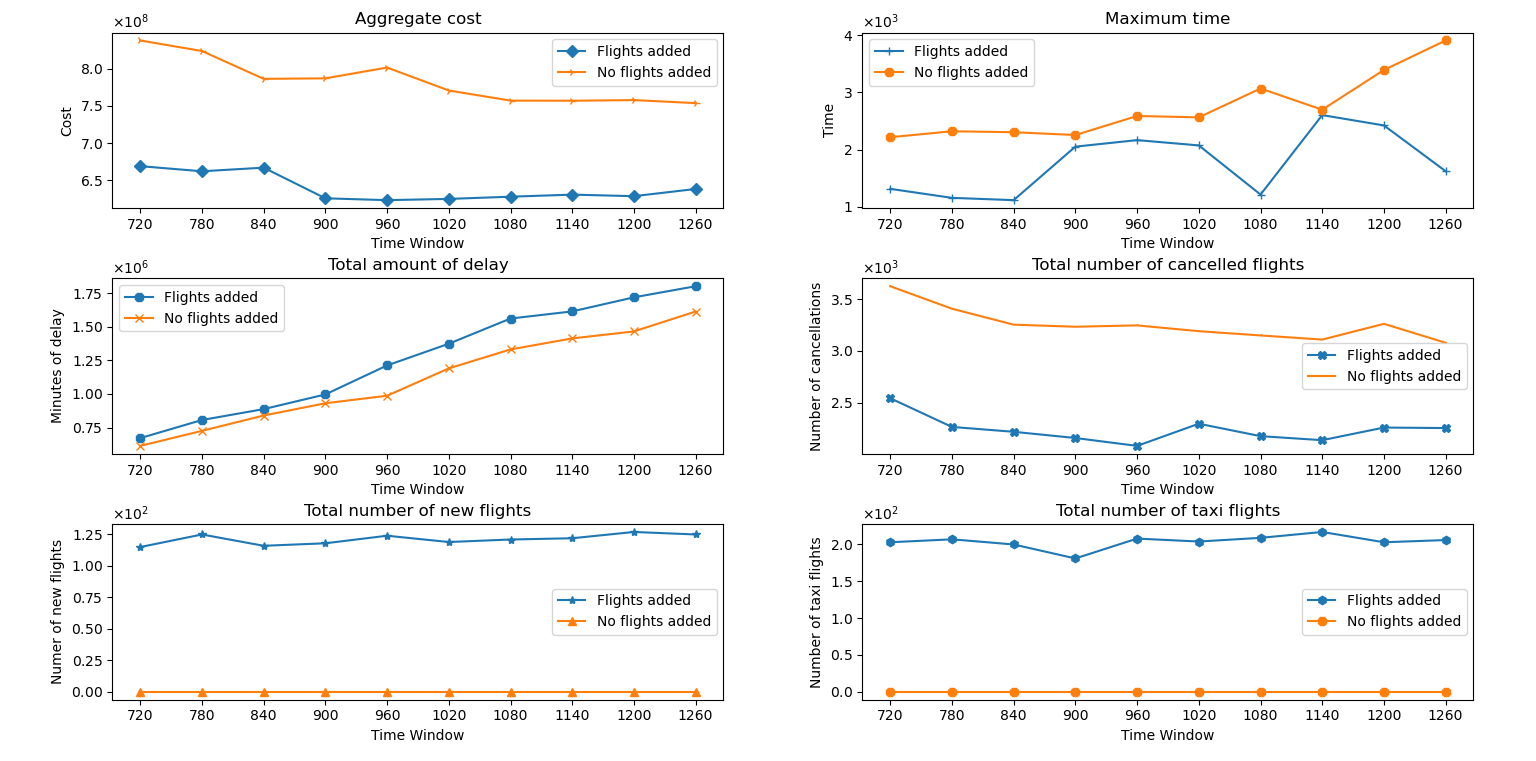
\includegraphics[width=\textwidth]{figures/flightNoFlight2x3.png}
		\caption[]{Impact of New Flights and Taxi Flights}
		\label{fig:flightNoFlight}
	\end{figure}

Regarding the addition of new flights, we verify  that the best results are obtained for the time windows of 780 for "Flights added", and for the 900 minutes for "Only new flights", as shown in figure \ref{fig:costTimeFlights}. The maximum number of taxi flights occurs for the 960 minutes time window.\\

 In figure \ref{fig:costTimeFlights} we draw the Pareto Front and we verify the best results are for the time 840 and 900 minutes time  windows.

	\begin{figure}[h!]
		\centering
		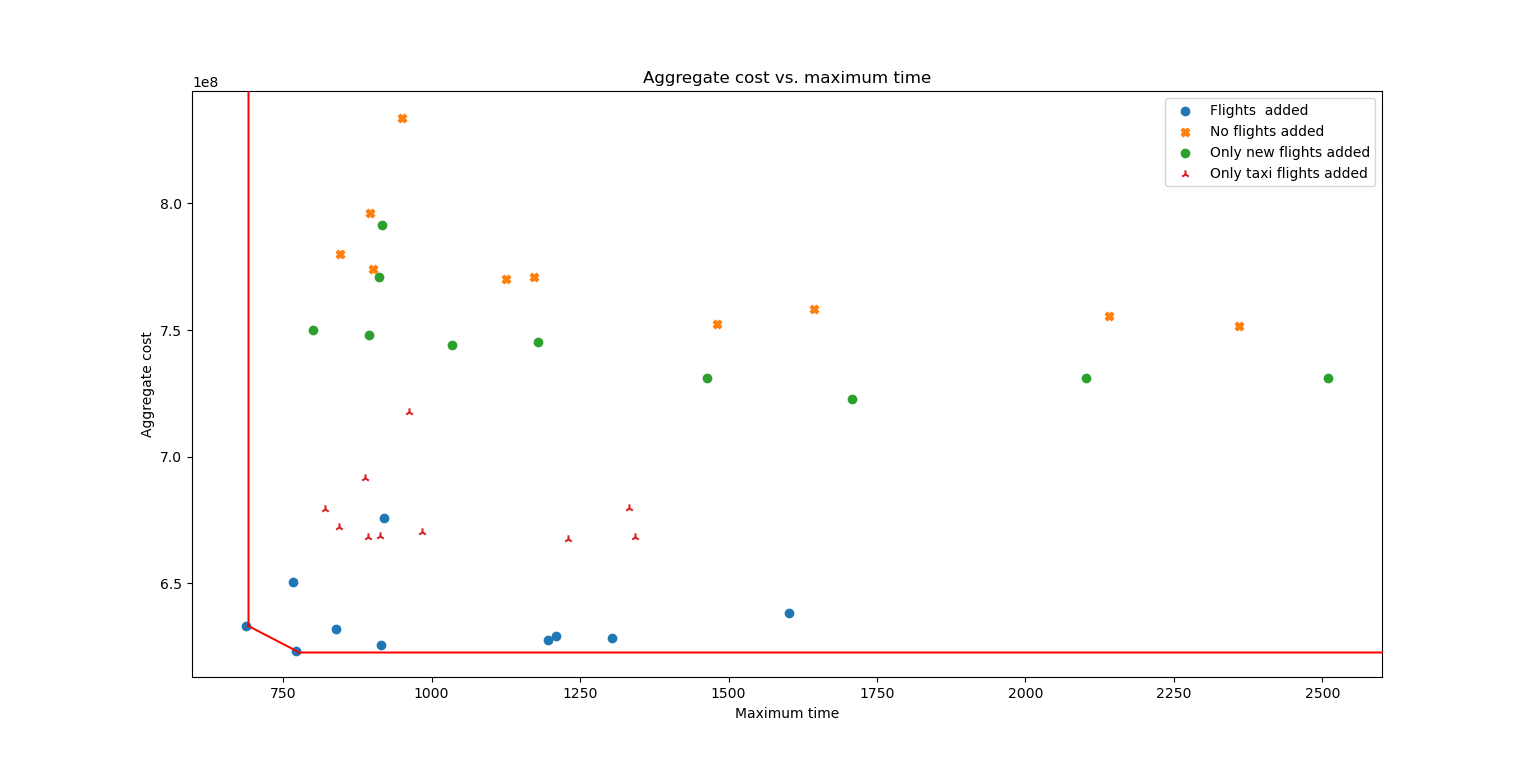
\includegraphics[width=\textwidth]{figures/costTimeFlights.png}
		\caption[]{Pareto Front for the Impact New Flights and Taxi Flights}
		\label{fig:costTimeFlights}
	\end{figure}



\subsection{Impact of the Pincer Speed}\label{sec:pincerSpeed}
To study the impact of the pincer speed we define the set of incremental and decremental steps in table \ref{tbl:pincerSpeed}.

	\begin{table}[h!]
		\centering
		\caption{Base Scenario}
		\label{tbl:pincerSpeed}
		\begin{tabular}{lll}
			\hline
			& Incremental step size     & Decremental step size      \\
			Speed 0.5 & $0.5 \times 10^{4}$ & $0.5 \times 10^{11}$ \\
			Speed 1   & $1.0 \times 10^{4}$ & $1.0 \times 10^{11}$ \\
			Speed 2   & $2.0 \times 10^{4}$ & $2.0 \times 10^{11}$ \\
			Speed 3   & $3.0 \times 10^{4}$ & $3.0 \times 10^{11}$ \\
			Speed 4   & $4.0 \times 10^{4}$ & $4.0 \times 10^{11}$ \\
			Speed 5   & $5.0 \times 10^{4}$ & $5.0 \times 10^{11}$ \\
			Speed 6   & $6.0 \times 10^{4}$ & $6.0 \times 10^{11}$ \\
			\hline
		\end{tabular}
	\end{table} 
The incremental and decremental are used in figure \ref{fig:mainAlgo} in step  13 to update the lower and upper bound in each iteration of the CHARP.
Since in Subsection \ref{sec:impact} we proved that "Flights added" has the best results, in this Subsection we will this configuration to study the impact of the pincer speed.\\

 In figure \ref{fig:speed} we can observe that the minimum aggregate cost and computing time is obtained for speed 5 in the 900 minutes times window. For the total amount of delay we observe that it increases with the time window and that the different speeds observe the same pattern of behaviour. In relation to the total number of flight cancellations we can observe that the values have a sharp decrease from 720 to 780 minutes, after which they stabilize between a minimum of 2083 at speed 1 for the 960 minutes time window  and a maximum of 2351 at speed 6 for the time window of 1200 minutes. As for the number of new flights we can observe that they increase steadily with the size of the time window. Finally, in relation to the number of taxi flights other than a sharp decrease in value for the time window of 900 minutes, the remaining values distribute themselves between 195 at speed 4 for the 1200 minutes time window and 226 at speed 3 for the 1020 minutes time window.
 
	\begin{figure}[h!]
		\centering
		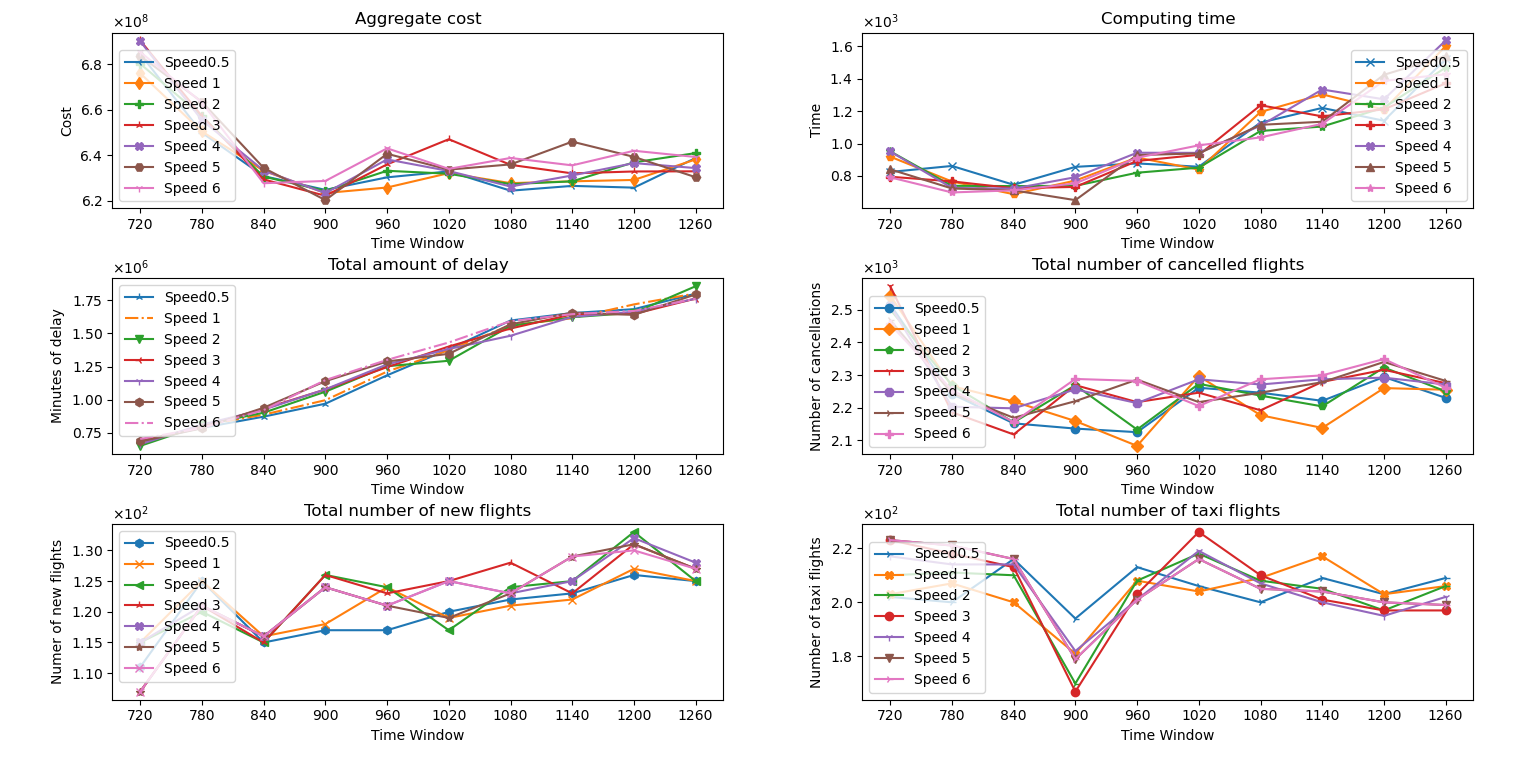
\includegraphics[width=\textwidth]{figures/speed.png}
		\caption[]{Impact of the Pincer Speed}
		\label{fig:speed}
	\end{figure}

To have a better understanding of the solution quality in figure \ref{fig:costTimeSpeed} we draw the Pareto front considering the aggregate cost versus the computing time for the different speeds and we the best result is for speed 5.

	\begin{figure}[h!]
		\centering
		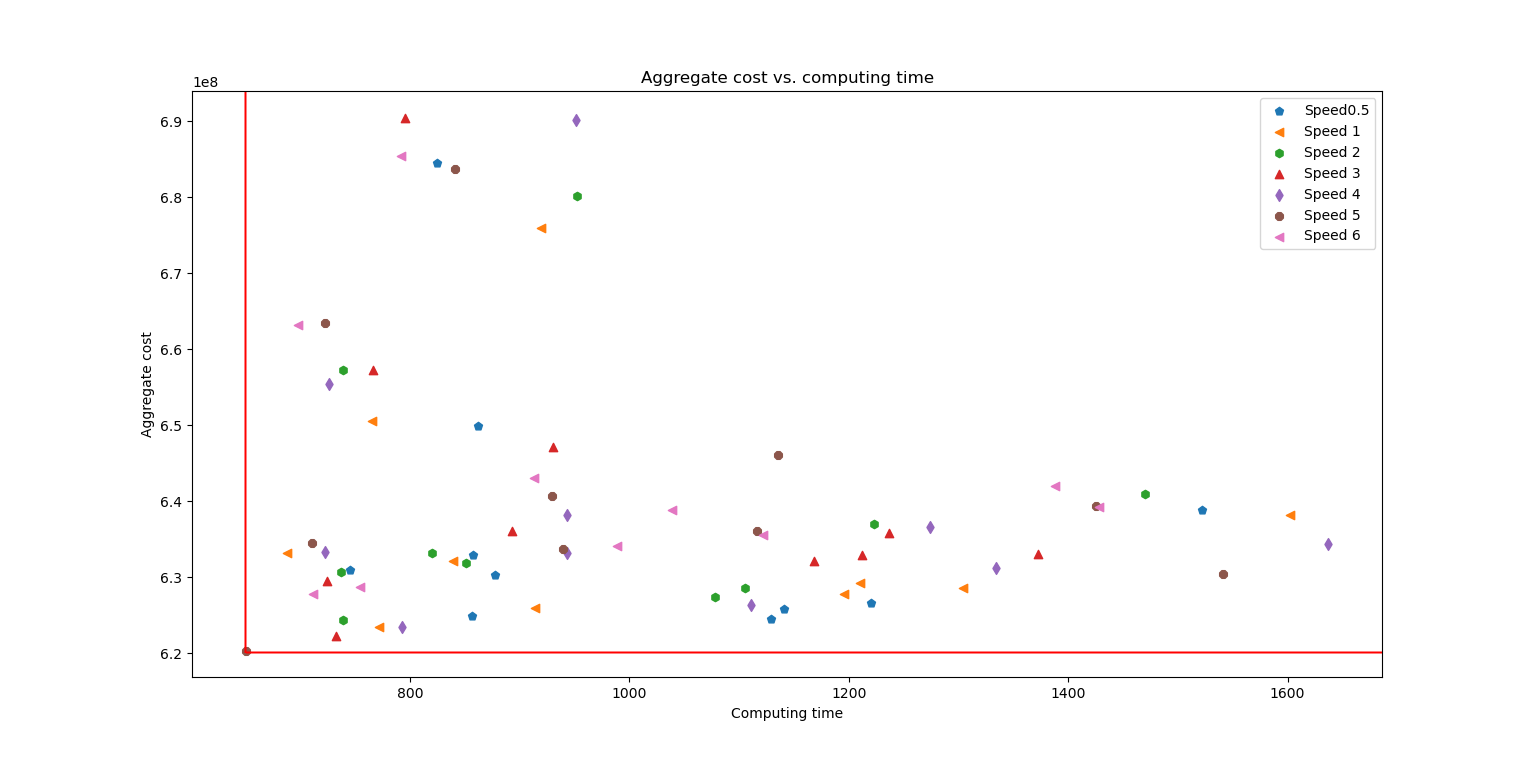
\includegraphics[width=\textwidth]{figures/costTimeSpeed.png}
		\caption[]{The Pareto Front for the Pincer Heuristic speed change}
		\label{fig:costTimeSpeed}
	\end{figure}

\subsection{Impact of the Step Size on the CHARP} \label{sec:stepSize}

In this section we study the impact of the step sizes 20 and 35 and since speed 5 had the best result we aim at observing if it is possible to make further improvement. As shown in figure \ref{fig:speed5Step} we confirm that the 60 minutes step shows the best result for the time window of 900 minutes.

	\begin{figure}[h!]
		\centering
		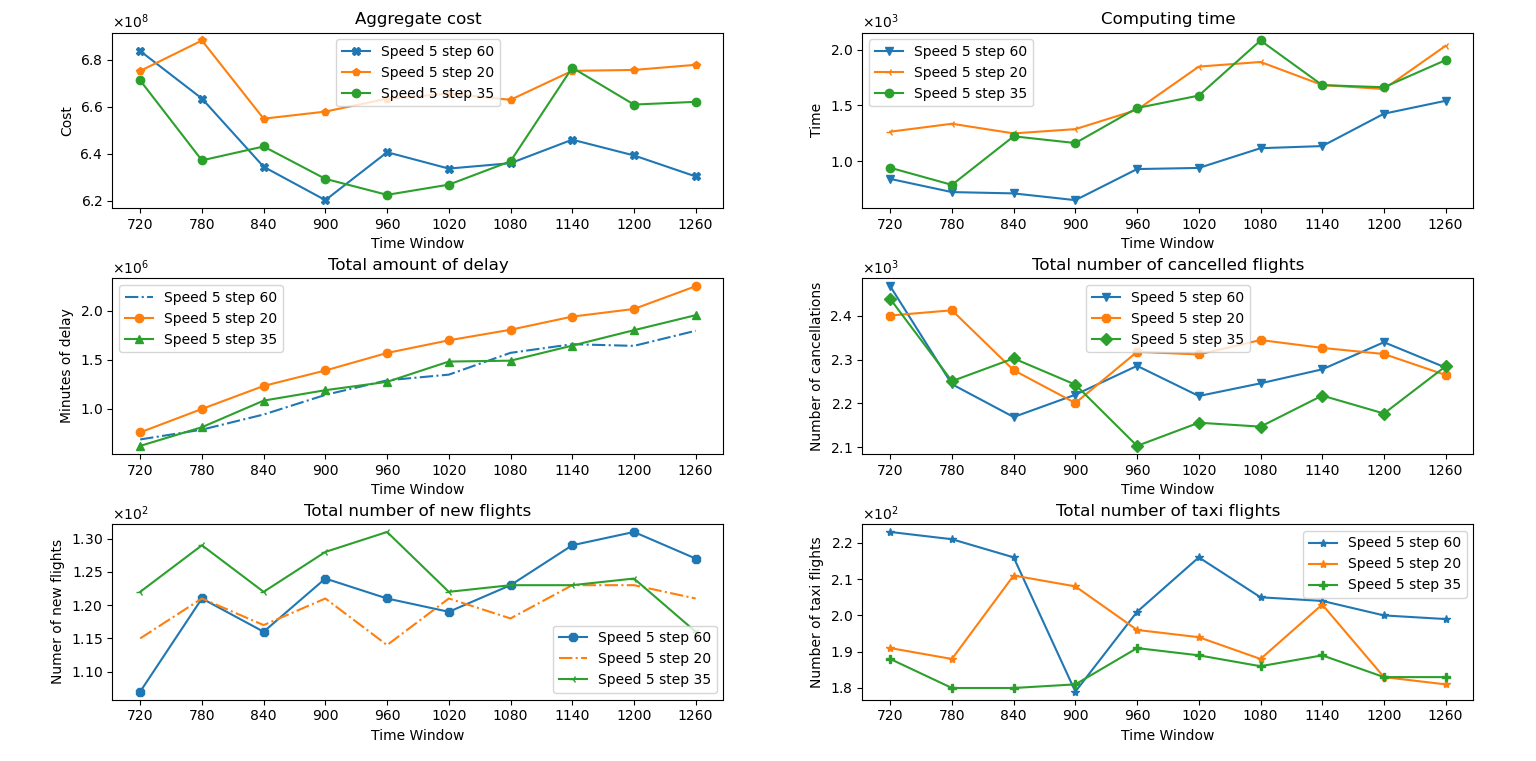
\includegraphics[width=\textwidth]{figures/speed5Step.png}
		\caption[]{Impact of the Step Size on the CHARP}
		\label{fig:speed5Step}
	\end{figure}

In figure \ref{fig:costTimeStep} we confirm the previous observation and we also notice that the computing time increases as the time time window increases.

	\begin{figure}[h!]
		\centering
		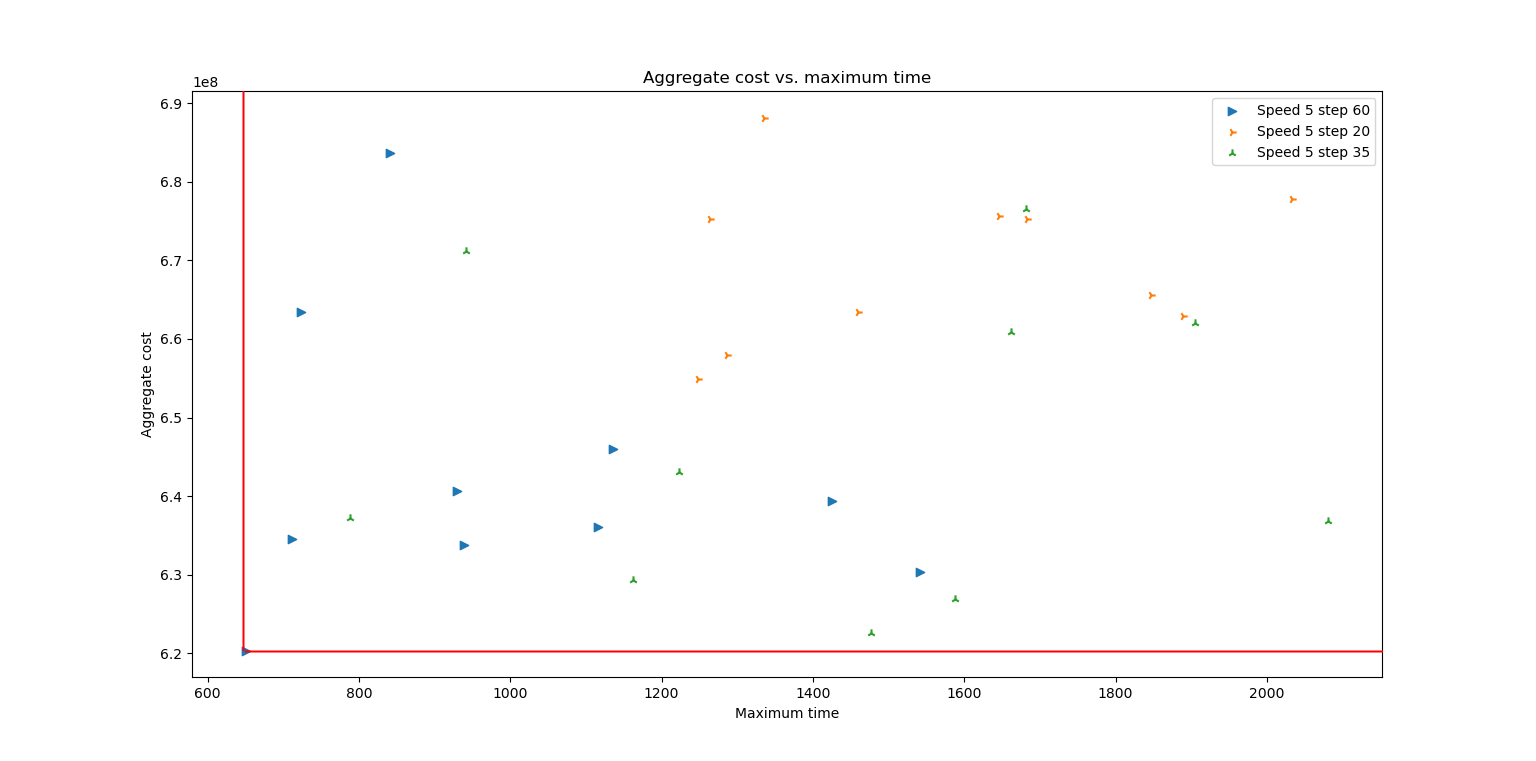
\includegraphics[width=\textwidth]{figures/costTimeStep.png}
		\caption[]{The Pareto Front for the Step Size on the CHARP}
		\label{fig:costTimeStep}
	\end{figure}